\pdfobjcompresslevel 0
\documentclass[a4paper,twoside,12pt]{book}
\usepackage[utf8]{inputenc}
\usepackage[T1]{fontenc}

\usepackage{listings,chngcntr}
%\lstset{frame=Trbl,numbers=left}

\usepackage{fancyvrb,xcolor}
\usepackage{moreverb}


\usepackage{amsmath}
\usepackage{amssymb}
\usepackage{mathrsfs}

\usepackage{graphicx}
\usepackage{multirow}
\usepackage{multicol}
\usepackage{algorithm,algorithmic}
\usepackage{pdfpages}
\usepackage{eqparbox,array}
\usepackage{longtable}
\usepackage[left=1in, right=1in, top=1in, bottom=1in, includefoot, headheight=28pt]{geometry}
%\usepackage{hyperref}
%\usepackage[left=3.5cm,right=2cm,top=2cm,bottom=2.5cm]{geometry}
%\pgfplotsset{compat=1.12}
%\usepackage[tableposition=top]{caption}

%%%%%%%%Chapter labels%%%%%
%1-	chapter_introduction
%2-	chapter_background
%3- 	chapter_graph_ordering_heuristics
%4- 	chapter_degree_aware_scheduling
%5-	chapter_state_of_the_art
%6- 	chapter_graph_dsls_improvement
%7- 	chapter_conclusion

\newcommand{\fonction}[5]
{
  \begin{array}{lrcl}
    #1:&#2& \rightarrow& #3 \\
    & #4&\mapsto&#5
  \end{array}
}

\newtheorem{theo}{\textbf{Theorem}}[section]
\newtheorem{prop}{\textbf{Property}}[section]
\newenvironment{proof}[1][Proof:]
{\begin{trivlist} \item[\hskip \labelsep  {\bfseries #1}]}
{\end{trivlist}}

\newenvironment{proofInd}[1][Proof indications:]
{\begin{trivlist} \item[\hskip \labelsep  {\bfseries #1}]}
{\end{trivlist}}

\renewcommand\algorithmiccomment[1]{%
  \hfill  \eqparbox{COMMENT}{\scriptsize \textit{#1}}%
}
\newcommand\LONGCOMMENT[1]{%
  \hfill\#\ \begin{minipage}[t]{\eqboxwidth{COMMENT}}#1\strut\end{minipage}%
}

\usepackage{url}
\usepackage{titling}

%opening
\title{Titre du mémoire}
\author{NOM1 Prénom1 matricule1, \\ NOM2 Prénom2 matricule2,  \\ NOM3 Prénom3 matricule3 \\Co-supervisor (Structure): Titre Nom Prénom\\ \ \ \ \ Co-supervisor (Structure): Titre NOM Prénom}


\linespread{1.3}

\begin{document}
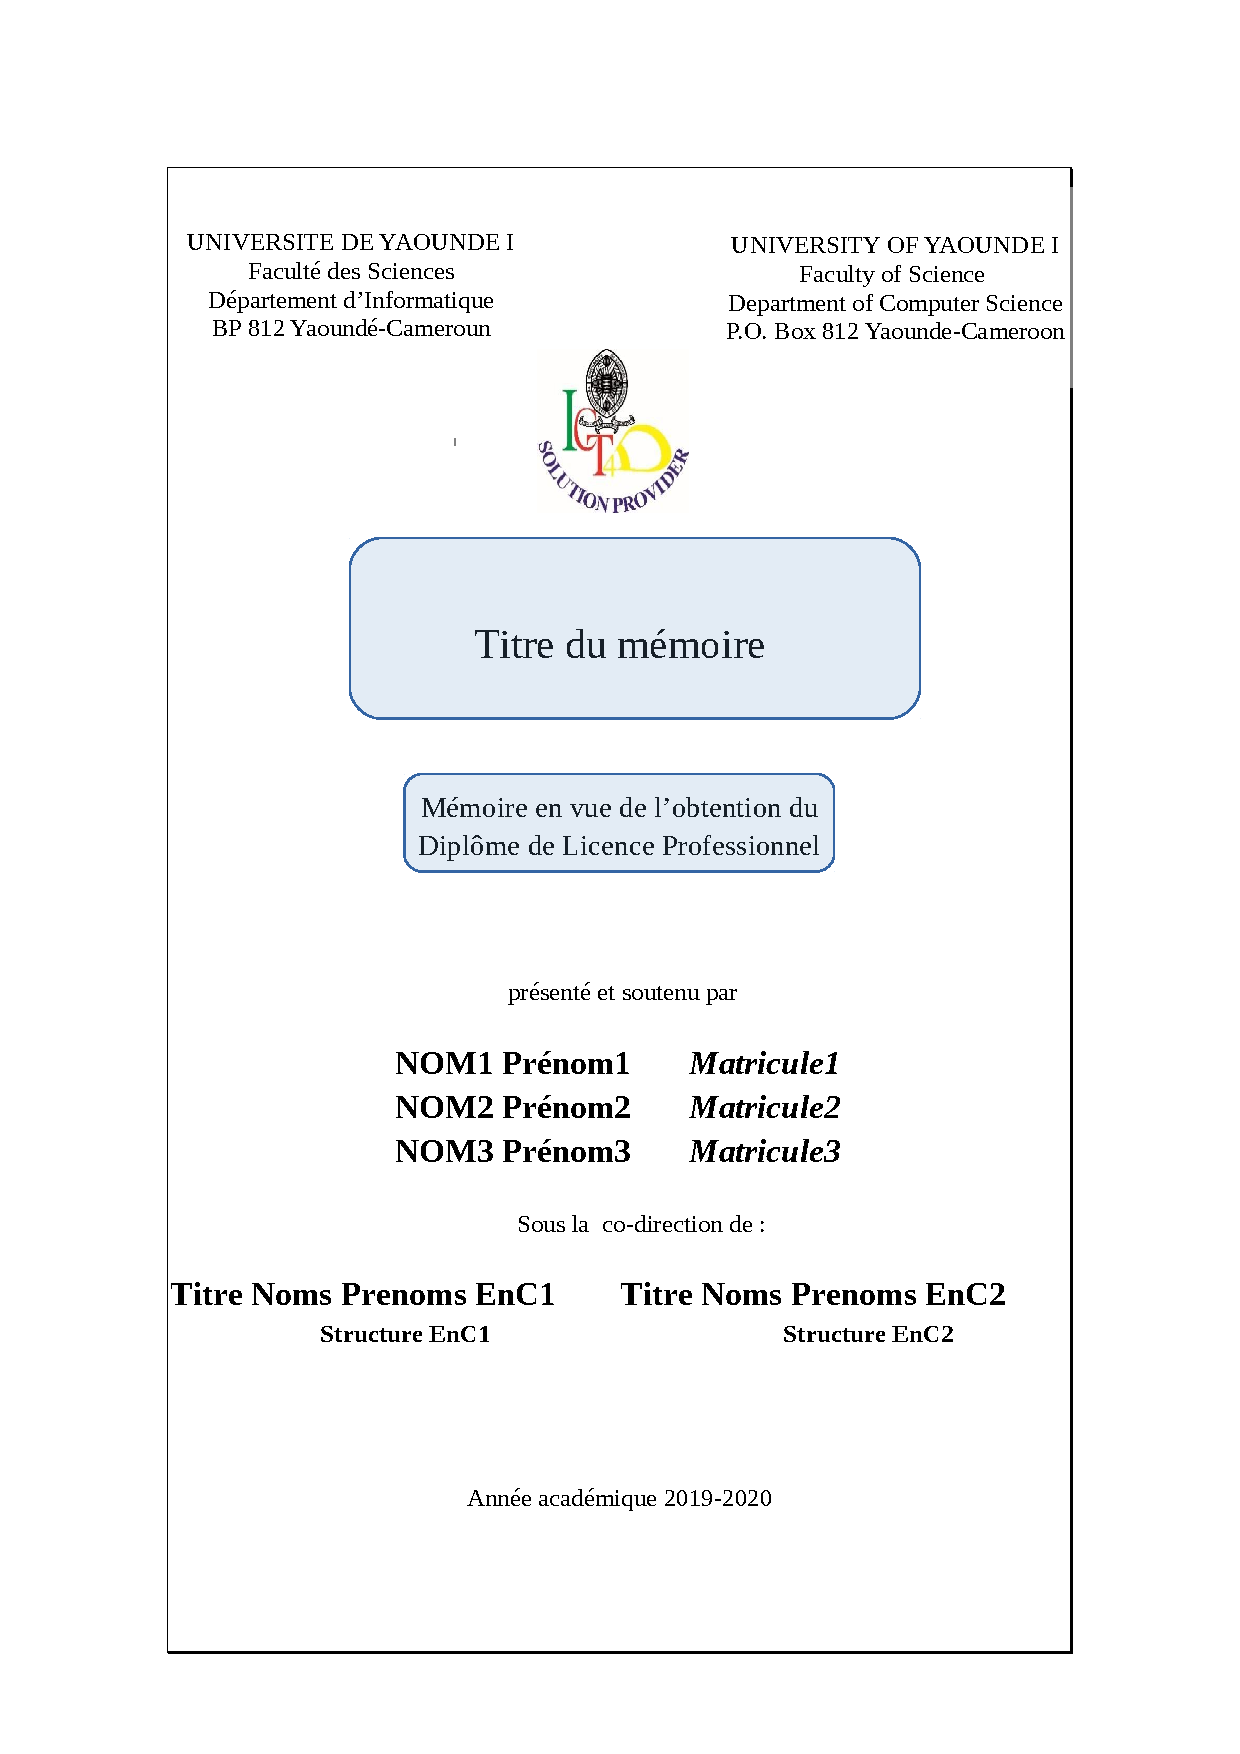
\includepdf[pages={1}]{couverture_memoire_ict_nom1_nom2_nom3.pdf}
\maketitle

\pagenumbering{roman}


{\fontsize{10.46}{13}\selectfont
\section*{Abstract}
Your abstract in english: Context, Problem to solve, Existing solutions, Proposed Solution, Results, Perspectives. 
%\end{abstract}
}
%\begin{abstract}
%\end{abstract}
\newpage
{\fontsize{10.46}{13}\selectfont
\section*{Résumé}

Resumé en français contenant le contexte, le problème à resourdre, les solutions existantes, la solution proposée, les resultats obtenus, les paerspectives.
}
\newpage
\ \\ \ \\ \ \\ \ \\ \ \\ \ \\ \ \\ \ \\ \ \\ \ \\ \ \\ \ \\ \ \\ \ \\ \ \\ \ \\
\begin{center}
\textit{
 To ...}
\end{center}

\newpage

\section*{Acknowledgements.}

I thank all of you who contributed to bring the accomplishment of this thesis. First of all, I thank you my supervisors, ...

Thank you ...

I thank ...

A special thank you to ...

My heartfelt gratitude to you my teachers of University of Yaounde I .....

I thank my colleagues and friends from Yaoundé ...

Finally, I thank you, ...

\newpage

\section*{Remerciements.}
Je vous remercie, vous tous qui de près ou de loin avez contribué à mener à terme cette thèse. En premier lieu, je vous remercie vous mes ...

Je vous remercie ... pour avoir accepté de participer à ce jury de thèse ...

Je remercie ...

Je vous remercie, vous les ...

Je vous remercie, vous mes enseignants de Yaoundé I ...

Je vous remercie, vous mes collègues et amis de Yaoundé ...


Je vous remercie enfin, vous les membres de ma famille: ...

\tableofcontents

%\tableoffigures

%\chapter*{Preface}

\pagenumbering{arabic}
% Chapter 1

\chapter{Introduction} % Main chapter title
\label{chapter_introduction}

\cite{messiarima}


Contexte, problème, solutions existantes, solution proposée, annonce du plan. 

% Chapter 1

\chapter{Background et état de l'art} % Main chapter title
\label{chapter_background} % For referencing the chapter elsewhere, use \ref{Chapter1}
On présente les solutions existantes et tout ce qu'il faut connaitre pour comprendre le mémoire.
\cite{messiarima}

\chapter[Agent virtuel: Chatbot]{Agent virtuel} % Main chapter title
\label{chapter_degree_aware_scheduling} % For referencing the chapter elsewhere, use \ref{Chapter1} 

\chapter[implémentation, expérimentation, resultat]{implémentation, expérimentation, resultat} % Main chapter title
\label{chapter_degree_aware_scheduling} % For referencing the chapter elsewhere, use \ref{Chapter1}

% Chapter 1

\chapter{Conclusion et perspective} % Main chapter title
\label{chapter_conclusion} % For referencing the chapter elsewhere, use \ref{Chapter1} 

Ici on rappelle le contexte, le problème, la solution proposée, les resultats obtenus, et les perspectives.


\bibliographystyle{plain}
\bibliography{bibli}
\appendix
\chapter{Titre de l'annexe 1 ...}

\end{document}
